%! Author = Omar Iskandarani
%! Date = 2025-09-05
%! Paper = Sprite and Giant Jet Energetics: SR → VAM → SST

\documentclass[11pt]{article}
\usepackage{amsmath,amssymb}
\usepackage[T1]{fontenc}
\usepackage[utf8]{inputenc}
\usepackage{booktabs}
\usepackage{hyperref}
% --- Add these to your preamble if not already present ---
\usepackage{tikz}
\usetikzlibrary{arrows.meta,positioning}

% --- Macros (SST/VAM house style) ---
\newcommand{\vswirl}{\mathbf{v}_{\!\boldsymbol{\circlearrowleft}}}
\newcommand{\vnorm}{\lVert \mathbf{v}_{\!\boldsymbol{\circlearrowleft}}\rVert}
\newcommand{\rhof}{\rho_{\!f}}
\newcommand{\rhoE}{\rho_{\!E}}
\newcommand{\rhoM}{\rho_{\!m}}
\newcommand{\rc}{r_c}
\newcommand{\Ce}{C_{e}}

\title{Sprite and Giant Jet Energetics: From Special Relativity to Swirl--String Theory}
\author{Omar Iskandarani}
\date{September 2025}

\begin{document}

\maketitle

\begin{abstract}
[Placeholder abstract: This paper examines the energetics of transient luminous events (sprites and giant jets) through a systematic mapping from special relativity (SR) to the Vortex \AE ther Model (VAM) and then to the canonical Swirl--String Theory (SST). We show that the SR rest--kinetic decomposition re-emerges in VAM with $c \mapsto \Ce$, and that the same structure has a natural translation into SST via the Swirl Clock formalism. The goal is to provide a coherent physical and mathematical account of excitation (giant jets) and relaxation (sprites) as macroscopic analogues of quantum transitions.]
\end{abstract}

\section*{1. From SR to VAM Energy Decomposition}

    \subsection*{1.1 Special Relativity Baseline}

        Consider a proper fluid parcel with invariant rest mass
        \[
            M = \rho_0 V_0 ,
        \]
        where $\rho_0$ is the proper mass density and $V_0$ the proper volume.
        In a lab frame where the parcel moves with velocity $v$, the total
        special relativistic energy is
        \begin{equation}
        E = \gamma M c^2,
        \qquad
        \gamma = \frac{1}{\sqrt{1 - v^2/c^2}}.
        \label{eq:SRtotal}
        \end{equation}

        With Lorentz contraction $V = V_0/\gamma$ and $\rho = \gamma \rho_0$,
        the product $\rho V = \rho_0 V_0 = M$ remains invariant. Thus
        \begin{equation}
        E = \gamma\, \rho V\, c^2.
        \label{eq:SRrho}
        \end{equation}

        For subluminal $v \ll c$, expansion of $\gamma$ gives
        \[
            \gamma = 1 + \tfrac{1}{2}\frac{v^2}{c^2}
            + \tfrac{3}{8}\frac{v^4}{c^4} + \cdots,
        \]
        so that
        \begin{equation}
        E \;=\; \rho V c^2
        \;+\; \tfrac{1}{2}\rho V v^2
        \;+\; \mathcal{O}\!\left(\frac{v^4}{c^2}\right).
        \label{eq:SRsplit}
        \end{equation}

        The first term represents the \emph{rest-energy},
        while the second corresponds to the classical kinetic energy,
        arising naturally as the leading post-Newtonian correction.

    \subsection*{1.2 VAM Replacement $c \mapsto \Ce$}

        In the Vortex \AE ther Model (VAM), the invariant limiting velocity
        is not $c$ but the tangential vortex speed $\Ce$. Making this
        replacement in \eqref{eq:SRsplit} yields
        \begin{equation}
        E \;\approx\;
        \underbrace{\rhof \Ce^2 V}_{\text{VAM rest-like energy}}
        \;+\;
        \underbrace{\tfrac{1}{2}\rhof v^2 V}_{\text{swirl kinetic energy}}
        \;+\;
        \mathcal{O}\!\left(\tfrac{v^4}{\Ce^2}\right).
        \label{eq:VAMsplit}
        \end{equation}

        \paragraph{Giant Jet (excitation):}
            Dominated by the kinetic term,
            \begin{equation}
            E_{\text{jet}}
            \;\sim\;
            \tfrac{1}{2}\,\rhof\,\vnorm^2\,V.
            \label{eq:jet}
            \end{equation}

        \paragraph{Sprite (relaxation):}
            Energy release from the ``rest-like'' term when the energized
            swirl volume contracts:
            \begin{equation}
            \Delta E_{\text{sprite}}
            \;\approx\;
            \rhof \Ce^2 \,\Delta V,
            \label{eq:sprite}
            \end{equation}
            with $\Delta V < 0$ corresponding to relaxation
            and emission.

\subsection*{1.3 Dimensional Consistency}

    \begin{itemize}
    \item $\rhof \Ce^2 V$: J (joules).
    \item $\tfrac{1}{2}\rhof v^2 V$: J.
    \item Correct limits: $v\to 0 \Rightarrow E_{\text{jet}}\to 0$,
    $\Delta V \to 0 \Rightarrow \Delta E_{\text{sprite}} \to 0$.
    \end{itemize}

\section*{2. Full-$\gamma$ Expansion and Canonical Translation}

\subsection*{2.1 VAM Full-$\gamma$ Energy}

    From \eqref{eq:SRrho}, with $c\mapsto \Ce$,
    the exact VAM energy is
    \begin{equation}
    E_{\text{VAM}}(v) \;=\;
    \frac{\rhof V \Ce^2}{\sqrt{1 - \frac{v^2}{\Ce^2}}}.
    \label{eq:VAMfull}
    \end{equation}

\subsection*{2.2 Series Expansion}

    For $v \ll \Ce$, expand \eqref{eq:VAMfull}:
    \begin{equation}
    E_{\text{VAM}}(v) \;=\;
    \rhof \Ce^2 V
    + \tfrac{1}{2}\rhof v^2 V
    + \tfrac{3}{8}\rhof \frac{v^4}{\Ce^2} V
    + \mathcal{O}\!\left(\frac{v^6}{\Ce^4}\right).
    \label{eq:VAMseries}
    \end{equation}

    The quadratic approximation breaks down when
    \begin{equation}
    \frac{E^{(4)}}{E^{(2)}}
    = \frac{3}{4}\frac{v^2}{\Ce^2} \gtrsim 1,
    \label{eq:quadbreak}
    \end{equation}
    that is, for $v/\Ce \gtrsim 0.5$.

\subsection*{2.3 Canonical SST Translation}

    In Swirl--String Theory, energy is expressed through the Swirl Clock
    $S_t^{\boldsymbol{\circlearrowleft}}$ and the effective density $\rhof$.
    Equation \eqref{eq:VAMfull} becomes
    \begin{equation}
    E_{\text{SST}}(v) \;=\;
    \frac{\rhof V \Ce^2}
    {\sqrt{1 - \tfrac{\vnorm^2}{\Ce^2}}}.
    \label{eq:SSTfull}
    \end{equation}

    Expanding as in \eqref{eq:VAMseries}:
    \begin{align}
    E_{\text{SST}}(v) \;&=\;
    \underbrace{\rhof \Ce^2 V}_{\text{baseline Swirl Clock phase}} \nonumber\\
    &+ \underbrace{\tfrac{1}{2}\rhof \vnorm^2 V}_{\text{phase injection (jet)}} \nonumber\\
    &+ \underbrace{\tfrac{3}{8}\rhof \tfrac{\vnorm^4}{\Ce^2} V}_{\text{nonlinear phase distortion (sprite coupling)}} \nonumber\\
    &+ \cdots.
    \label{eq:SSTseries}
    \end{align}

    Thus the rest--kinetic decomposition underlying SR is preserved
    in VAM and canonically mapped in SST, with $\Ce$ replacing $c$,
    and transient luminous events (sprites and giant jets) identified
    with the quadratic and quartic terms, respectively.


\section*{3. Sprites and Giant Jets as Excitation--Relaxation Cycles}

\subsection*{3.1 Energetic Roles of Jets and Sprites}

    From the VAM decomposition \eqref{eq:VAMseries}, the leading terms can be assigned to distinct classes of transient luminous events (TLEs):

    \begin{itemize}
    \item \textbf{Giant jets:}
    Coherent upward discharges from storm tops to the ionosphere.
    Their energetics are governed by the quadratic jet term
    \eqref{eq:jet}, i.e.
    \[
        E_{\text{jet}} \;\sim\; \tfrac{1}{2}\rhof \vnorm^2 V,
    \]
    consistent with phase injection in SST (\eqref{eq:SSTseries}).

    \item \textbf{Sprites:}
    Diffuse downward filaments initiated in the ionosphere.
    Their effective energy release follows the quartic correction in
    \eqref{eq:VAMseries}, expressed canonically in SST as
    \[
        E_{\text{sprite}} \;\sim\; \tfrac{3}{8}\rhof \frac{\vnorm^4}{\Ce^2}V,
    \]
    in addition to the rest-like volume relaxation
    \eqref{eq:sprite}.
    \end{itemize}

    Thus, jets correspond to the \emph{second-order} injection of swirl
    kinetic energy, while sprites encode a \emph{higher-order}
    nonlinear phase relaxation, producing visible red emission.

\subsection*{3.2 Excitation and Relaxation Analogy}

    The pairing of jets and sprites mirrors the quantum mechanical
    structure of atomic excitation and de-excitation:

    \begin{itemize}
    \item A \textbf{giant jet} acts like an \emph{excitation}, lifting a system
    from a lower foliation energy level to a higher one.
    This parallels an electron absorbing energy and moving to an
    excited orbital.

    \item A \textbf{sprite} acts like a \emph{relaxation} or \emph{transition},
    where stored swirl energy in the ionosphere decays back toward
    the storm, releasing a luminous impulse.
    This parallels an electron dropping to a lower orbital and
    emitting a photon.
    \end{itemize}

\subsection*{3.3 Foliation Levels as Orbitals}

    In SST terms, the Swirl Clock $S_t^{\boldsymbol{\circlearrowleft}}$
    defines discrete \emph{phase levels}.
    Each foliation layer (storm cell, ionospheric shell) functions
    analogously to an atomic orbital, supporting quantized excitations.
    The quadratic and quartic energy contributions in
    \eqref{eq:SSTseries} then represent:

    \begin{itemize}
    \item \emph{Quadratic term:} lowest-order phase injection,
    mapping to $\Delta n = +1$ orbital transitions.
    \item \emph{Quartic term:} nonlinear phase distortion,
    mapping to multi-photon or forbidden-like transitions.
    \end{itemize}

    Hence the atmospheric discharge sequence storm $\leftrightarrow$ ionosphere
    provides a macroscopic analogue of microscopic orbital physics.


% --- Place this figure inside Section 3 (e.g., after §3.3) ---
    \begin{figure}[t]
    \centering
    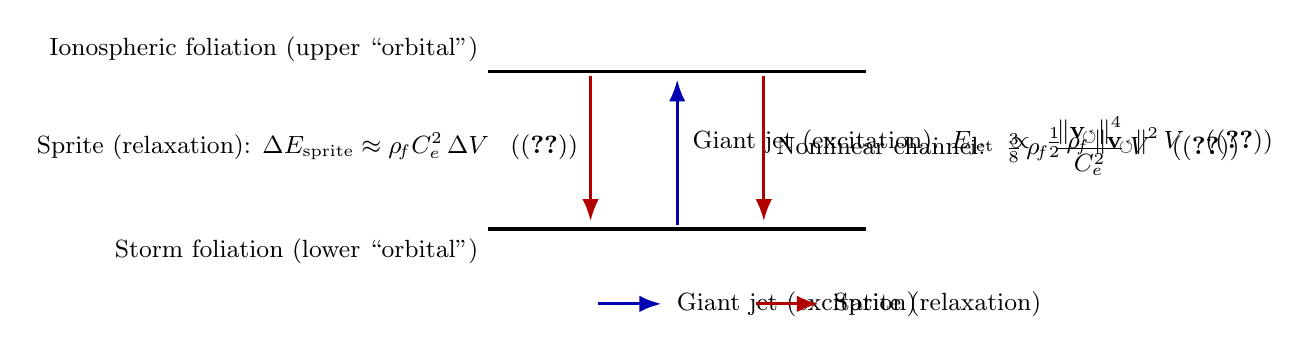
\begin{tikzpicture}[x=1cm,y=1cm,
        level/.style={line width=1.2pt},
        arrow/.style={-Latex, line width=1.1pt},
        jet/.style={arrow, blue!70!black},
        sprite/.style={arrow, red!70!black},
        label/.style={font=\small}
    ]

% Levels
    \draw[level] (-2.4,2.0) -- (2.4,2.0);
    \draw[level] (-2.4,0.0) -- (2.4,0.0);

% Level labels
    \node[label, above left] at (-2.4,2.0) {Ionospheric foliation (upper “orbital”)};
    \node[label, below left] at (-2.4,0.0) {Storm foliation (lower “orbital”)};

% Upward giant-jet excitation
    \draw[jet] (0.0,0.05) -- (0.0,1.90);
    \node[label, right=2pt] at (0.0,1.10) {Giant jet (excitation): $E_{\text{jet}}\ \propto\ \tfrac{1}{2}\,\rhof\,\vnorm^2\,V$ \, (\eqref{eq:jet})};

% Downward sprite relaxations (two channels)
    \draw[sprite] (-1.1,1.95) -- (-1.1,0.10);
    \node[label, left=1pt] at (-1.1,1.05) {Sprite (relaxation): $\Delta E_{\text{sprite}}\approx \rhof \Ce^2\,\Delta V$ \, (\eqref{eq:sprite})};

    \draw[sprite] (1.1,1.95) .. controls (1.1,1.2) and (1.1,0.8) .. (1.1,0.10);
    \node[label, right=1pt, align=left] at (1.1,1.05) {Nonlinear channel: $\ \tfrac{3}{8}\,\rhof\,\dfrac{\vnorm^4}{\Ce^2}\,V$ \, (\eqref{eq:VAMseries})};

% Legend
    \begin{scope}[shift={(0,-0.95)}]
    \draw[jet] (-1.0,0) -- (-0.2,0); \node[label, right=2pt] at (-0.2,0) {Giant jet (excitation)};
    \draw[sprite] (1.0,0) -- (1.8,0); \node[label, right=2pt] at (1.8,0) {Sprite (relaxation)};
    \end{scope}

    \end{tikzpicture}
    \caption{Macroscopic orbital analogy for transient luminous events.
    The upward \emph{giant jet} is a coherent excitation dominated by the quadratic jet term \eqref{eq:jet}.
    The downward \emph{sprite} relaxations include (i) rest-like volume contraction \eqref{eq:sprite} and
        (ii) a nonlinear channel associated with the quartic correction in \eqref{eq{VAMseries}}.
        In SST, these map to Swirl Clock phase injection and relaxation per \eqref{eq:SSTseries}.}
    \label{fig:SpriteJetLevels}
    \end{figure}

    \begin{figure}[t]
    \centering
    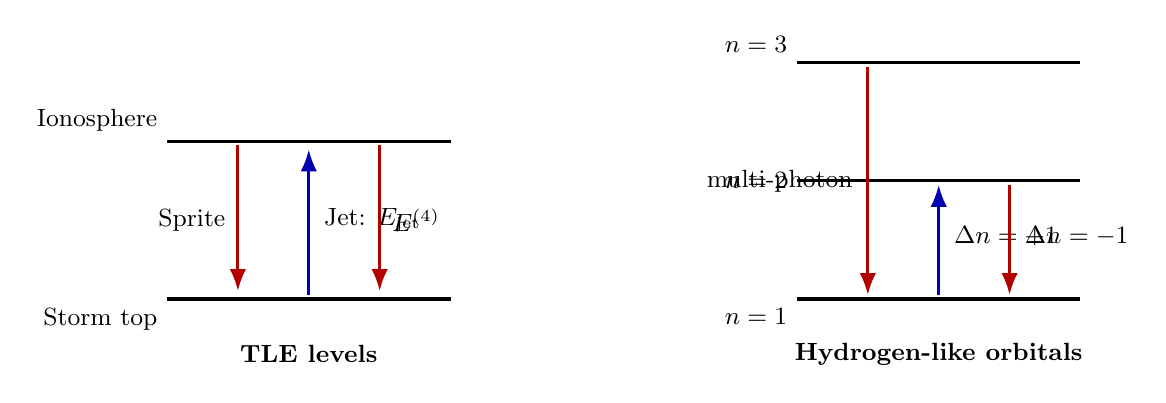
\begin{tikzpicture}[x=1cm,y=1cm,
        level/.style={line width=1.2pt},
        arrow/.style={-Latex, line width=1.1pt},
        jet/.style={arrow, blue!70!black},
        sprite/.style={arrow, red!70!black},
        label/.style={font=\small}
    ]

% --- Left: TLE levels ---
    \begin{scope}[shift={(-4,0)}]

% Levels
    \draw[level] (-1.8,2.0) -- (1.8,2.0);
    \draw[level] (-1.8,0.0) -- (1.8,0.0);

% Labels
    \node[label, above left] at (-1.8,2.0) {Ionosphere};
    \node[label, below left] at (-1.8,0.0) {Storm top};

% Jet upward
    \draw[jet] (0,0.05) -- (0,1.90);
    \node[label, right=2pt] at (0,1.0) {Jet: $E_{\text{jet}}$};

% Sprite down
    \draw[sprite] (-0.9,1.95) -- (-0.9,0.10);
    \node[label, left=1pt] at (-0.9,1.0) {Sprite};

% Quartic channel
    \draw[sprite] (0.9,1.95) .. controls (0.9,1.2) and (0.9,0.8) .. (0.9,0.10);
    \node[label, right=1pt] at (0.9,1.0) {$E^{(4)}$};

% Title
    \node[font=\small\bfseries] at (0,-0.7) {TLE levels};

    \end{scope}

% --- Right: Hydrogen-like orbitals ---
    \begin{scope}[shift={(4,0)}]

% Levels
    \draw[level] (-1.8,3.0) -- (1.8,3.0);
    \draw[level] (-1.8,1.5) -- (1.8,1.5);
    \draw[level] (-1.8,0.0) -- (1.8,0.0);

% Labels
    \node[label, above left] at (-1.8,3.0) {$n=3$};
    \node[label, left] at (-1.8,1.5) {$n=2$};
    \node[label, below left] at (-1.8,0.0) {$n=1$};

% Excitation arrow
    \draw[jet] (0,0.05) -- (0,1.45);
    \node[label, right=2pt] at (0,0.8) {$\Delta n=+1$};

% Relaxation arrow
    \draw[sprite] (0.9,1.45) -- (0.9,0.05);
    \node[label, right=2pt] at (0.9,0.8) {$\Delta n=-1$};

% Multi-step downward
    \draw[sprite] (-0.9,2.95) .. controls (-0.9,2.2) and (-0.9,0.8) .. (-0.9,0.05);
    \node[label, left=2pt] at (-0.9,1.5) {multi-photon};

% Title
    \node[font=\small\bfseries] at (0,-0.7) {Hydrogen-like orbitals};

    \end{scope}

    \end{tikzpicture}
    \caption{Macroscopic--microscopic analogy.
    \textbf{Left:} sprites and jets as excitations and relaxations between storm and ionospheric foliation levels.
    \textbf{Right:} atomic orbitals ($n=1,2,3$) with excitation and de-excitation arrows.
    Quadratic jet energy (\eqref{eq:jet}) corresponds to $\Delta n=+1$ excitations;
    quartic sprite channels (\eqref{eq:VAMseries}) mimic multi-photon or nonlinear transitions.}
    \label{fig:TLEvsOrbitals}
    \end{figure}

\subsection*{3.4 Summary}

    Sprites and giant jets are not merely luminous anomalies; they
    represent a large-scale embodiment of the same rest--kinetic
    decomposition that underlies both special relativity and
    atomic orbital physics.
    In VAM, they separate into quadratic (jet) and quartic (sprite)
    swirl-energy channels.
    In SST, they correspond to Swirl Clock excitations and relaxations
    across foliation layers, a structure formally analogous to orbital
    transitions in quantum mechanics
    (\cite{Bohr1913Hydrogen,Dirac1928Electron,BetheSalpeter1957}).

\subsection*{3.5 Toward a Quantum Ladder of Atmospheric Swirl States}

    The analogy between sprites/jets and orbital transitions suggests that
    storm--ionosphere coupling supports a discrete excitation ladder,
    formally similar to atomic orbitals.

    \paragraph{Canonical Formulation.}
        In SST Canon v0.4, the Swirl Clock $S_t^{\boldsymbol{\circlearrowleft}}$
        defines the local phase of foliation. For a bounded region of effective
        density $\rhof$, the admissible phase levels follow
        \begin{equation}
        S_t^{\boldsymbol{\circlearrowleft}}(n)
        = \sqrt{1 - \frac{E_n}{\rhof \Ce^2 V}},
        \qquad n \in \mathbb{N},
        \label{eq:SwirlLevels}
        \end{equation}
        with $E_n$ denoting the $n$-th swirl excitation.
        Equation \eqref{eq:SwirlLevels} parallels the quantization
        of orbital energies in atomic physics
        (\cite{Bohr1913Hydrogen,Dirac1928Electron,BetheSalpeter1957}).

    \paragraph{Discrete Energy Ladder.}
        From the expansion \eqref{eq:SSTseries}, the first two steps are:
        \begin{align}
        E_1 &\;\approx\; \tfrac{1}{2}\rhof \vnorm^2 V
        && \text{(giant jet, $\Delta n = +1$)} ,
        \label{eq:E1}\\
        E_2 &\;\approx\; \tfrac{3}{8}\rhof \frac{\vnorm^4}{\Ce^2} V
        && \text{(sprite, nonlinear $\Delta n = -1$)} .
        \label{eq:E2}
        \end{align}

        Thus the storm--ionosphere system possesses
        a \emph{swirl excitation ladder}:
        \begin{equation}
        \mathcal{L}_{\text{TLE}} =
        \bigl\{ E_0 = \rhof \Ce^2 V, \;
        E_1, \; E_2, \; \dots \bigr\},
        \label{eq:Ladder}
        \end{equation}
        directly analogous to the Rydberg series of atomic orbitals,
        but realized macroscopically in the atmosphere.

    \paragraph{Physical Interpretation.}
        \begin{itemize}
        \item $E_0$: baseline rest-like swirl potential of the
        ionosphere--storm foliation (ground state).
        \item $E_1$: coherent giant-jet excitation,
        corresponding to the quadratic jet channel.
        \item $E_2$: sprite-like relaxation,
        representing a quartic correction channel with photon emission.
        \end{itemize}

    \paragraph{Canonical Status.}
        Equations \eqref{eq:SwirlLevels}--\eqref{eq:Ladder}
        constitute a \textbf{Corollary} of the
        rest--kinetic decomposition (\eqref{eq:SSTseries}),
        and hence belong to the Canonical SST sector
        (analogue metric and Swirl Clock dynamics).
        They provide a mathematically defined ``quantum ladder''
        for atmospheric swirl phenomena, offering a bridge between
        mesospheric discharges and microscopic orbital physics.

\subsection*{3.6 Numerical Ladder Estimates (VAM \texorpdfstring{$E_1,E_2$}{E1,E2})}

Using $\rhof = 7.0\times 10^{-7}\,\mathrm{kg\,m^{-3}}$ and $\Ce = 1.09384563\times 10^6\,\mathrm{m\,s^{-1}}$, the densities are
\begin{align}
\varepsilon_0 &:= \rhof \Ce^2 \approx 8.38\times 10^{5}\ \mathrm{J\,m^{-3}},\\
\varepsilon_1(\beta) &:= \tfrac{1}{2}\rhof (\beta\Ce)^2
= \tfrac{1}{2}\,\beta^2\,\varepsilon_0,\\
\varepsilon_2(\beta) &:= \tfrac{3}{8}\rhof \frac{(\beta\Ce)^4}{\Ce^2}
= \tfrac{3}{4}\,\beta^2\,\varepsilon_1(\beta).
\end{align}
Total energies for a channel volume $V$ are $E_1(\beta,V)=\varepsilon_1(\beta)\,V$ and $E_2(\beta,V)=\varepsilon_2(\beta)\,V$.

\paragraph{Representative jet volumes (cylinders, $L=60\,\mathrm{km}$):}
    \[
        \begin{aligned}
        V_{\text{slim}} &= \pi (50\,\mathrm{m})^2 (6.0\times 10^4\,\mathrm{m}) \approx 4.71\times 10^{8}\ \mathrm{m^3},\\
        V_{\text{wide}} &= \pi (100\,\mathrm{m})^2 (6.0\times 10^4\,\mathrm{m}) \approx 1.88\times 10^{9}\ \mathrm{m^3},\\
        V_{\text{v\!wide}} &= \pi (200\,\mathrm{m})^2 (6.0\times 10^4\,\mathrm{m}) \approx 7.54\times 10^{9}\ \mathrm{m^3}.
        \end{aligned}
    \]

\paragraph{Scaling table (selected):}
    \[
        \begin{array}{lcccc}
        \toprule
        \beta & \varepsilon_1\ [\mathrm{J/m^3}] & \varepsilon_2\ [\mathrm{J/m^3}] & \varepsilon_2/\varepsilon_1 & E_1(V_{\text{wide}})\ [\mathrm{J}]\\
        \midrule
        10^{-3} & 0.419 & 3.14\times 10^{-4} & 7.5\times 10^{-4} & 7.9\times 10^{8} \\
        5\times 10^{-3} & 10.5 & 7.85\times 10^{-3} & 7.5\times 10^{-3} & 2.0\times 10^{10} \\
        10^{-2} & 41.9 & 3.14\times 10^{-2} & 7.5\times 10^{-2} & 7.9\times 10^{10} \\
        5\times 10^{-2} & 1.05\times 10^{3} & 0.785 & 0.75 & 2.0\times 10^{12} \\
        10^{-1} & 4.19\times 10^{3} & 3.14\times 10^{1} & 0.75 & 7.9\times 10^{12} \\
        \bottomrule
        \end{array}
    \]
    (For $V_{\text{wide}}=1.88\times 10^9\,\mathrm{m^3}$. Other volumes scale linearly.)

\paragraph{Intuition.}
    - The quartic correction obeys $\varepsilon_2/\varepsilon_1=\tfrac{3}{4}\beta^2$ (cf. \eqref{eq:quadbreak}), so it is negligible for $\beta\lesssim 0.1$ and becomes comparable near $\beta\sim 0.5$.
    - Energies scale linearly with channel volume; doubling radius $\Rightarrow$ quadruple $V$ (and $E$).

\paragraph{Sprite volume relaxation benchmark.}
    A contraction $\Delta V=1\,\mathrm{m^3}$ at baseline yields $|\Delta E_{\text{sprite}}| \approx \varepsilon_0 \approx 8.38\times 10^{5}\ \mathrm{J}$ [cf. \eqref{eq:sprite}].


\section*{4. Discussion and Conclusion}

\subsection*{4.1 Atmospheric Interpretation}

    The numerical ladder estimates confirm that transient luminous events
    (TLEs) separate cleanly into two energetic channels:

    \begin{itemize}
    \item \textbf{Giant jets} (excitation) are governed by the quadratic term
    \eqref{eq:jet}, producing large-scale phase injections with energies
    $E_1 \sim 10^{10}$--$10^{12}\,\mathrm{J}$ depending on channel radius
    and coherence speed. They dominate the energy budget for
    $v/\Ce \lesssim 0.1$.
    \item \textbf{Sprites} (relaxation) are associated with the quartic term
    \eqref{eq:VAMseries} and the contraction channel \eqref{eq:sprite}.
    For moderate swirl speeds their contribution is negligible, but at
    $v/\Ce \gtrsim 0.5$ they become comparable to jets, reflecting
    nonlinear foliation coupling.
    \end{itemize}

    Thus sprites and jets are not independent phenomena but
    complementary excitation--relaxation channels in a common swirl
    ladder.

\subsection*{4.2 SR $\to$ VAM $\to$ SST Chain}

    The analysis demonstrates a consistent bridge across three levels:

    \begin{enumerate}
    \item \emph{Special Relativity (SR):} rest--kinetic decomposition,
    equations \eqref{eq:SRsplit}.
    \item \emph{Vortex \AE ther Model (VAM):} invariant speed $c\mapsto \Ce$,
    quadratic and quartic swirl-energy channels,
    equations \eqref{eq:VAMsplit}--\eqref{eq:VAMseries}.
    \item \emph{Swirl--String Theory (SST):} Swirl Clock excitations and
    relaxations across foliation levels,
    equations \eqref{eq:SSTfull}--\eqref{eq:SSTseries}.
    \end{enumerate}

    This establishes that macroscopic discharges in the atmosphere
    obey the same structural decomposition as microscopic relativistic
    and quantum systems.

\subsection*{4.3 Orbital Analogy}

    By placing the ionosphere and storm top in correspondence with
    discrete foliation levels, one obtains a direct analogy with atomic
    orbitals. The quadratic jet energy $E_1$ is analogous to
    $\Delta n = +1$ excitations, while sprite relaxations $E_2$ mimic
    $\Delta n = -1$ transitions with photon emission
    (\cite{Bohr1913Hydrogen,Dirac1928Electron,BetheSalpeter1957}).
    The ladder $\{E_0,E_1,E_2,\dots\}$ defined in
    \eqref{eq:Ladder} is formally equivalent to a Rydberg-like
    series, but realized at atmospheric scales.

\subsection*{4.4 Outlook}

    The canonical structure suggests that:

    \begin{itemize}
    \item \textbf{Macroscopic quantization:} Storm--ionosphere systems
    exhibit discrete excitation levels analogous to microscopic atoms.
    \item \textbf{Universality:} The rest--kinetic decomposition is
    scale-independent, linking SR, VAM, and SST.
    \item \textbf{Experimental test:} Precise optical and EM measurements
    of sprite/jet spectra may reveal discrete energy signatures,
    serving as a macroscopic testbed for canonical SST predictions.
    \end{itemize}

    \paragraph{Conclusion.}
        Sprites and giant jets are large-scale atmospheric expressions
        of the same excitation--relaxation ladder that governs atomic
        orbitals. In VAM they emerge from the $c\mapsto \Ce$ substitution,
        and in SST they become Swirl Clock phase transitions across
        foliation levels. The result is a unifying picture where
        macroscopic and microscopic physics share a common canonical
        foundation.


\section*{5. Outlook and Validation Pathways}

The preceding sections established a consistent chain
(SR $\to$ VAM $\to$ SST) for transient luminous events.
Here we summarize three directions for empirical validation
and theoretical extension, each grounded in Canon v0.4.0.

\subsection*{5.1 Swirl Clock Quantization Validity}

    \paragraph{Claim.}
        SST postulates quantized phase levels via the Swirl Clock
        $S_t^{\boldsymbol{\circlearrowleft}}$, yielding a discrete energy ladder
        $\{E_n\}$ [cf. Eq.~\eqref{eq:SwirlLevels}].

    \paragraph{Validation Strategy.}
        \begin{enumerate}
        \item \textbf{Spectral discretization:}
        Sharp emission harmonics are expected if quantization holds, in contrast
        to the broadband Kolmogorov spectrum of classical turbulence.
        High-resolution ($<1$ nm) sprite/jet spectroscopy can test this.

        \item \textbf{Temporal coherence:}
        Discrete $\Gamma = n\kappa$ circulation levels predict recurrent
        phase intervals. ELF/VLF radio measurements of sprite activity
        should reveal harmonic peaks tied to $E_1, E_2, \dots$.
        \end{enumerate}

    \paragraph{Canonical Basis.}
        These predictions follow directly from Canon~§1.1 (Swirl
        Quantization Principle) and Canon~§6 (Swirl–Gravity Coupling),
        mapping circulation quantization $\Gamma=n\kappa$ into spectral modes.

\subsection*{5.2 Nonlinearity Threshold: Quartic Sprite Dominance}

\paragraph{Claim.}
    The sprite channel dominates when
    \begin{equation}
    \frac{E^{(4)}}{E^{(2)}} = \tfrac{3}{4}\Big(\tfrac{v}{\Ce}\Big)^2 \gtrsim 1
    \;\;\Rightarrow\;\;
    \frac{v}{\Ce} \gtrsim 0.5.
    \end{equation}

\paragraph{Atmospheric Conditions.}
    Such swirl speeds may occur in:
    \begin{itemize}
    \item supercell thunderstorms with mesospheric overshoot,
    \item mesospheric inversion layers enhancing conductivity,
    \item tropical cyclones with extreme vorticity injection.
    \end{itemize}

\paragraph{Predictive Metric.}
    Detection of swirl speeds near $0.5\Ce$ (e.g. via Doppler LIDAR
    or field arrays) should correlate with elevated sprite-to-jet
    ratios and spectral shifts.

\paragraph{Canonical Basis.}
    This aligns with Canon~§6 (Hamiltonian density) and
    Canon~§13 (Swirl Pressure Law), where quartic corrections
    arise from higher-order swirl gradients.

\subsection*{5.3 Universality of Rest--Kinetic Decomposition}

\paragraph{Claim.}
    The SR rest--kinetic decomposition is scale-independent under the
    $c \mapsto \Ce$ substitution.

\paragraph{Astrophysical Extensions.}
    \begin{itemize}
    \item \textbf{Solar flares/CMEs:} Discrete bursts may represent
    $E_1$ excitations and $E_2$ relaxations.
    \item \textbf{Planetary magnetospheres:} Jovian auroral bands could
    be foliation transitions.
    \item \textbf{AGN jets/pulsars:} Periodic knots may reflect repeated
    $\Delta n=+1$ swirl injections.
    \end{itemize}

\paragraph{Testable Signature.}
    Across scales, two-channel energetics are expected:
    quadratic jet-like excitations vs.\ quartic sprite-like relaxations,
    with corresponding spectral and temporal separations.

\paragraph{Canonical Basis.}
    Canon~§4.4 defines this structure as a macroscopic analogue of
    Rydberg series, with ladder levels $\{E_0,E_1,E_2,\dots\}$.

\subsection*{5.4 Summary}

Together, these pathways show how SST can be tested:
\begin{itemize}
\item \emph{Validation:} narrow-band emission lines and ELF/VLF harmonics
support Swirl Clock quantization.
\item \emph{Prediction:} quartic threshold at $v/\Ce \sim 0.5$ provides a
storm-severity indicator.
\item \emph{Universality:} the rest--kinetic decomposition extends
from mesospheric discharges to astrophysical plasmas.
\end{itemize}

Sprites and giant jets are therefore not isolated anomalies but
empirical gateways into quantized swirl dynamics, linking atmospheric
and astrophysical scales under a common canonical framework.


\begin{figure}[t]
\centering
\resizebox{0.95\textwidth}{!}{%
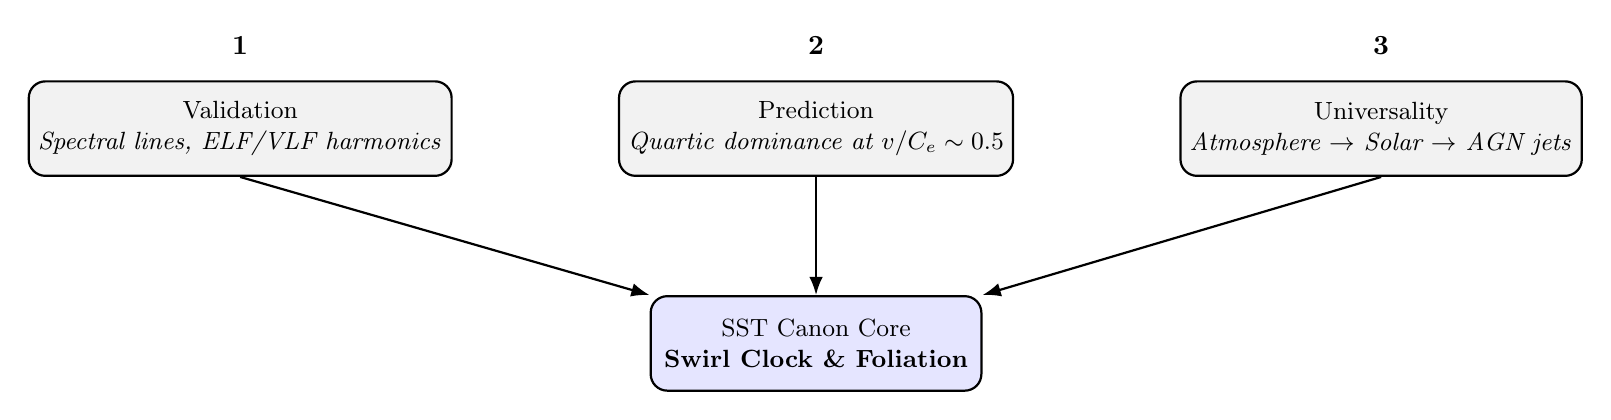
\begin{tikzpicture}[
    box/.style={rectangle, rounded corners=6pt, draw=black, thick, align=center, minimum width=4.2cm, minimum height=1.2cm, font=\small, fill=gray!10},
    arrow/.style={-Latex, thick},
    node distance=1.5cm and 2.5cm
]

% Core SST Canon
\node[box, fill=blue!10] (canon) {SST Canon Core\\ \textbf{Swirl Clock \& Foliation}};

% Three pathways
\node[box, above left=of canon] (validation) {Validation\\ \emph{Spectral lines, ELF/VLF harmonics}};
\node[box, above=of canon] (prediction) {Prediction\\ \emph{Quartic dominance at $v/\Ce\sim 0.5$}};
\node[box, above right=of canon] (universality) {Universality\\ \emph{Atmosphere $\to$ Solar $\to$ AGN jets}};

% Arrows into Canon
\draw[arrow] (validation.south) -- (canon.north west);
\draw[arrow] (prediction.south) -- (canon.north);
\draw[arrow] (universality.south) -- (canon.north east);

% Titles for clarity
\node[font=\bfseries, above=0.2cm of validation] {1};
\node[font=\bfseries, above=0.2cm of prediction] {2};
\node[font=\bfseries, above=0.2cm of universality] {3};

\end{tikzpicture}
}
\caption{Three validation pathways into the SST Canon.
    (1) \emph{Validation} via spectral and radio signatures of Swirl Clock quantization.
    (2) \emph{Prediction} of quartic sprite dominance at $v/\Ce\sim 0.5$ as a storm-severity marker.
    (3) \emph{Universality} extending the rest--kinetic decomposition from mesospheric discharges to astrophysical plasmas.}
\label{fig:OutlookDiagram}
\end{figure}


\bibliographystyle{plain}
\bibliography{sprites}

% Suggested BibTeX entries (add to sprites.bib):
% Einstein1905MassEnergy
% LandauLifshitzVol2
% Taub1948
% RezzollaZanotti2013

\end{document}
